\documentclass[aspectratio=169]{beamer}

% Shared Beamer settings for Applied Machine Learning lectures (UPES).
% Keep this file free of \documentclass to allow reuse via \input.

% Allow lecture sources to use shared theme/assets without copying them into each lecture folder.
% NOTE: These paths are relative to `Unit-xx/Lecture-yy/latex/` (and `Lab/Experiment-xx/latex/`).
\makeatletter
\def\input@path{{../../../_shared/}{../../../_shared/UPES-Beamer-Theme/}}
\makeatother

\usetheme{UPES}
\setbeamertemplate{navigation symbols}{}

\usepackage{amsmath}
\usepackage{amssymb}
\usepackage{booktabs}
\usepackage{graphicx}
\usepackage{hyperref}
\usepackage{xcolor}
\usepackage{listings}

% Code listings (Python-oriented for this subject).
\lstset{
  language=Python,
  basicstyle=\ttfamily\small,
  keywordstyle=\color{blue},
  commentstyle=\color{gray},
  stringstyle=\color{teal},
  showstringspaces=false,
  columns=fullflexible,
  breaklines=true
}

\usepackage{tikz}
\usetikzlibrary{arrows.meta,positioning,shapes.geometric,calc,fit,backgrounds}

% Per-slide source line (references shown on the slide itself).
\newcommand{\slidesources}[1]{%
  \vfill
  {\tiny\color{gray}\raggedright\sloppy\parbox{\linewidth}{Sources: #1}\par}%
}

% Unit-wise source strings for this subject (used by slides/notes).
% Path is relative to the lecture `latex/` folder (the compilation CWD).
% Source strings for Applied Machine Learning (CSAI2017P) — used by slides + notes.
% Prescribed texts and reference books are taken from the course syllabus.
% Support texts are the author-hosted open-access editions:
%   statlearning.com            (ISL with Python)
%   probml.github.io/pml-book   (Murphy, Probabilistic Machine Learning)
%   d2l.ai                      (Dive into Deep Learning)
%   mml-book.github.io          (Mathematics for Machine Learning)

\newcommand{\AMLRepoURL}{https://github.com/tali7c/Applied-Machine-Learning}

% --- prescribed -------------------------------------------------------------
\newcommand{\AMLPrescribed}{%
M\"uller and Guido, \textit{Introduction to Machine Learning with Python}, O'Reilly, 2016.;%
Bishop, \textit{Pattern Recognition and Machine Learning}, Springer, 2006.;%
Murphy, \textit{Machine Learning: A Probabilistic Perspective}, MIT Press, 2012.;%
Han, Kamber and Pei, \textit{Data Mining: Concepts and Techniques} (3e), Morgan Kaufmann, 2012.%
}

% --- unit-wise ---------------------------------------------------------------
\newcommand{\AMLUnitISources}{%
M\"uller and Guido, \textit{Introduction to Machine Learning with Python}, Ch. 1.;%
Bishop, \textit{Pattern Recognition and Machine Learning}, Ch. 1.;%
Murphy, \textit{Probabilistic Machine Learning: An Introduction}, MIT Press, 2022, Ch. 1.;%
Mitchell, \textit{Machine Learning}, McGraw Hill, 1997, Ch. 1.;%
Scikit-learn documentation, accessed 2026-08-04.%
}

\newcommand{\AMLUnitIISources}{%
Bishop, \textit{Pattern Recognition and Machine Learning}, \S1.5, \S4.3, \S7.1.;%
Zhang, Lipton, Li and Smola, \textit{Dive into Deep Learning}, \S3.4.;%
Shalev-Shwartz and Ben-David, \textit{Understanding Machine Learning}, Ch. 15.;%
Murphy, \textit{Probabilistic Machine Learning: An Introduction}, Ch. 5.%
}

\newcommand{\AMLUnitIIISources}{%
Zhang, Lipton, Li and Smola, \textit{Dive into Deep Learning}, Ch. 12 (Optimization Algorithms).;%
Deisenroth, Faisal and Ong, \textit{Mathematics for Machine Learning}, Ch. 7.;%
Kingma and Ba, ``Adam: A Method for Stochastic Optimization,'' ICLR 2015.;%
Ruder, ``An overview of gradient descent optimization algorithms,'' arXiv:1609.04747, 2016.%
}

\newcommand{\AMLUnitIVSources}{%
Han, Kamber and Pei, \textit{Data Mining: Concepts and Techniques} (3e), Ch. 3.;%
M\"uller and Guido, \textit{Introduction to Machine Learning with Python}, Ch. 3--4.;%
James, Witten, Hastie, Tibshirani and Taylor, \textit{An Introduction to Statistical Learning with Python}, Ch. 5--6, 12.;%
Scikit-learn documentation (preprocessing, model selection), accessed 2026-08-04.%
}

\newcommand{\AMLUnitVSources}{%
James et al., \textit{An Introduction to Statistical Learning with Python}, Ch. 3--6.;%
Bishop, \textit{Pattern Recognition and Machine Learning}, Ch. 3.;%
Deisenroth, Faisal and Ong, \textit{Mathematics for Machine Learning}, Ch. 9.;%
M\"uller and Guido, \textit{Introduction to Machine Learning with Python}, \S2.3.%
}

\newcommand{\AMLUnitVISources}{%
Han, Kamber and Pei, \textit{Data Mining: Concepts and Techniques} (3e), Ch. 8--9.;%
James et al., \textit{An Introduction to Statistical Learning with Python}, Ch. 8--9.;%
Bishop, \textit{Pattern Recognition and Machine Learning}, Ch. 4--5, 7, 14.;%
Zhang et al., \textit{Dive into Deep Learning}, Ch. 5.%
}

\newcommand{\AMLUnitVIISources}{%
Han, Kamber and Pei, \textit{Data Mining: Concepts and Techniques} (3e), Ch. 10.;%
James et al., \textit{An Introduction to Statistical Learning with Python}, Ch. 12.;%
M\"uller and Guido, \textit{Introduction to Machine Learning with Python}, \S3.5.;%
Ester, Kriegel, Sander and Xu, ``A density-based algorithm for discovering clusters (DBSCAN),'' KDD 1996.%
}

\newcommand{\AMLLabSources}{%
M\"uller and Guido, \textit{Introduction to Machine Learning with Python}, companion notebooks.;%
McKinney, \textit{Python for Data Analysis} (3e), O'Reilly, 2022.;%
Scikit-learn user guide, accessed 2026-08-04.;%
Matplotlib and Seaborn documentation, accessed 2026-08-04.%
}



\graphicspath{{../figures/}{../images/}{../../../_shared/}{../../../_shared/UPES-Beamer-Theme/}}

\title[Applied Machine Learning]{Applied Machine Learning}
\subtitle{Unit 06 -- Lecture 16: Ensembles -- Bagging, Boosting and Random
Forests}
\author{Tofik Ali}
\institute{School of Computer Science, UPES Dehradun}
\date{Autumn 2026}

% ---- a compact "output" block so code and its result sit together ----------
\lstdefinestyle{outblk}{
  basicstyle=\ttfamily\scriptsize\color{black!75},
  backgroundcolor=\color{black!5}, frame=leftline, framerule=2pt,
  rulecolor=\color{black!30}, breaklines=true, columns=fullflexible,
  keepspaces=true,   % several outputs below are aligned tables
  language={},       % printed output is not Python: do not syntax-highlight it
  xleftmargin=4pt, aboveskip=1pt, belowskip=1pt, literate={-}{{-}}1}
\lstnewenvironment{outblk}{\lstset{style=outblk}}{}

\begin{document}

\UPESCoverFrame
\setcounter{framenumber}{0}

\begin{frame}
  \titlepage
  \begin{center}
    \footnotesize Why a committee of mediocre models beats a good one\\[0.25em]
    \footnotesize Topic focus: \textbf{diversity is the resource}\\[0.25em]
    \footnotesize Repository: \texttt{\AMLRepoURL}
  \end{center}
  \slidesources{\AMLUnitVISources}
\end{frame}

\begin{frame}{Quick Links}
  \centering
  \hyperlink{sec:why}{\beamerbutton{Why ensembles work}}\hspace{0.4em}
  \hyperlink{sec:bag}{\beamerbutton{Bagging}}\hspace{0.4em}
  \hyperlink{sec:var}{\beamerbutton{Variance, not bias}}\hspace{0.4em}
  \hyperlink{sec:rf}{\beamerbutton{Random forests}}\\[0.6em]
  \hyperlink{sec:imp}{\beamerbutton{Feature importance}}\hspace{0.4em}
  \hyperlink{sec:boost}{\beamerbutton{Boosting}}\hspace{0.4em}
  \hyperlink{sec:vs}{\beamerbutton{Bagging vs boosting}}\hspace{0.4em}
  \hyperlink{sec:summary}{\beamerbutton{Summary}}
\end{frame}

\begin{frame}{Agenda}
  \tableofcontents
\end{frame}

\begin{frame}[shrink=7]{How this lecture works}
  \begin{columns}[T]
    \begin{column}{0.48\textwidth}
      \begin{block}{Every idea appears twice}
        \begin{enumerate}
          \item \textbf{By hand} --- twenty-five voters, five rows in a hat,
            ten points on a line. Small enough that every number can be
            checked with a pen.
          \item \textbf{In code} --- the same arithmetic, then the same
            arithmetic again inside \texttt{scikit-learn}, so you can see
            the library is doing exactly this and nothing magic.
        \end{enumerate}
      \end{block}
    \end{column}
    \begin{column}{0.48\textwidth}
      \begin{alertblock}{Commit before you look}
        Five slides ask you to predict a number before it is revealed. Write
        your guess down. Being wrong on paper is how the idea sticks.
      \end{alertblock}
    \end{column}
  \end{columns}
  \vspace{0.4em}
  \begin{center}
    \small The centrepiece is \textbf{three rounds of AdaBoost worked on ten
    points}: the weighted error, the $\alpha$, the reweighting, and the
    combined sign. That arithmetic is the most examinable thing in the
    lecture.
  \end{center}
\end{frame}

\begin{frame}[shrink=5]{Where we are}
  \begin{columns}[T]
    \begin{column}{0.47\textwidth}
      \begin{block}{The decision-tree lecture left a problem}
        An unrestricted tree hits training accuracy $1.0000$ every time and
        then falls over on new rows. Pruning bought some of that back, but a
        single tree stayed \textbf{unstable}: move a few rows and the root
        split changes.
      \end{block}
      \begin{block}{This lecture turns that into an advantage}
        Instability means the trees you grow on slightly different data are
        \emph{different}. Average many different unstable models and the
        instability cancels.
      \end{block}
    \end{column}
    \begin{column}{0.49\textwidth}
      \begin{exampleblock}{Today's one question}
        I have a mediocre model. \emph{Can I build a good one out of many
        copies of it?}
      \end{exampleblock}
      \begin{alertblock}{And the answer has a condition}
        Yes --- provided the copies make their mistakes on
        \textbf{different rows}. Everything in this lecture is machinery for
        forcing them to disagree: resample the rows (\textbf{bagging}),
        restrict the features (\textbf{random forests}), or reweight the rows
        towards what is still wrong (\textbf{boosting}).
      \end{alertblock}
    \end{column}
  \end{columns}
\end{frame}

\begin{frame}[shrink=6]{One seed --- and the two things that are not it}
  \begin{columns}[T]
    \begin{column}{0.48\textwidth}
      \begin{block}{The one seed}
        \small Every arbitrary random choice in this deck uses
        \textbf{seed $0$}: \texttt{np.random.default\_rng(0)} or
        \texttt{random\_state=0}. Splits, bootstrap draws, flipped labels.
        Every listing that shuffles or samples shows it.
      \end{block}
      \begin{alertblock}{A seed that defines data}
        \small The three planted noise columns use
        \texttt{default\_rng(42)}. Change it and you have \emph{different
        data}, not a different experiment --- so it stays.
      \end{alertblock}
    \end{column}
    \begin{column}{0.48\textwidth}
      \begin{block}{A sweep}
        \small Twenty splits for out-of-bag, ten per noise level, with
        \texttt{random\_state=s} across the loop. Here the run-to-run
        variation \emph{is} the demonstration --- but the sweep starts at
        $0$, so it reproduces exactly too.
      \end{block}
      \begin{exampleblock}{Why this matters to you}
        \small Run the code as written and you get the numbers on the slide.
        That is the only reason to believe a number on a slide.
      \end{exampleblock}
    \end{column}
  \end{columns}
\end{frame}

% =====================================================================
\section[Why ensembles]{Why an ensemble beats its members}
\label{sec:why}

\begin{frame}[shrink=9]{An ensemble is a committee with a voting rule}
  \begin{exampleblock}{}
    \centering\large
    Train $m$ models. Ask all of them. Take the majority vote.
  \end{exampleblock}
  \vspace{0.3em}
  \begin{columns}[T]
    \begin{column}{0.48\textwidth}
      \begin{block}{The vocabulary}
        The individual models are the \textbf{base learners} or
        \textbf{members}. The rule that combines them is the
        \textbf{aggregation}: majority vote for classification, mean for
        regression, weighted versions of both.
      \end{block}
    \end{column}
    \begin{column}{0.48\textwidth}
      \begin{alertblock}{The claim to be justified}
        Twenty-five models that are each right $60\%$ of the time can be
        combined into one that is right about $85\%$ of the time --- the
        difference between a model you would throw away and one you would
        deploy.
      \end{alertblock}
    \end{column}
  \end{columns}
  \vspace{0.2em}
  \begin{center}\small
    The claim is a piece of eighteenth-century probability, not machine
    learning: \textbf{Condorcet's jury theorem}, 1785.
  \end{center}
\end{frame}

\begin{frame}{Predict first \#1 --- twenty-five mediocre voters}
  \begin{alertblock}{Commit to a number}
    Twenty-five classifiers. Each one is right $60\%$ of the time. Each one
    is \textbf{independent} of the others --- they get their answers wrong on
    unrelated rows. You take the majority vote.

    \medskip
    \centering\large
    What accuracy does the majority vote have?
  \end{alertblock}
  \onslide<2->{
  \begin{exampleblock}{}
    \centering\large
    $\Pr[\text{at least }13\text{ of }25\text{ correct}] = \mathbf{0.846232}$
  \end{exampleblock}
  \begin{center}\small
    A gain of $\mathbf{+0.2462}$ over any single member --- and every member
    is still only $60\%$ accurate. Nothing was improved. Only combined.
  \end{center}}
\end{frame}

\begin{frame}[shrink=4]{By hand: the binomial sum}
  Let $K$ be the number of members that get a given row right. Members are
  independent, so
  \[
    \Pr[K = k] = \binom{25}{k}\,(0.6)^k\,(0.4)^{25-k},
    \qquad
    \Pr[\text{vote correct}] = \sum_{k=13}^{25}\Pr[K=k].
  \]
  \begin{columns}[T]
    \begin{column}{0.44\textwidth}
      \begin{block}{The first few terms}
        \small
        \begin{tabular}{rrl}
          \toprule
          $k$ & $\binom{25}{k}$ & term \\
          \midrule
          13 & 5\,200\,300 & 0.11395006 \\
          14 & 4\,457\,400 & 0.14650722 \\
          15 & 3\,268\,760 & 0.16115794 \\
          16 & 2\,042\,975 & 0.15108557 \\
          \multicolumn{3}{c}{$\cdots$} \\
          25 & 1 & 0.00000284 \\
          \bottomrule
        \end{tabular}
      \end{block}
    \end{column}
    \begin{column}{0.52\textwidth}
      \begin{exampleblock}{The sum}
        $\sum_{k=13}^{25} = \mathbf{0.846232}$. The largest term is at
        $k = 15 = 0.6 \times 25$: the mode sits on the right of the majority
        threshold, so most of the mass lies above it.
      \end{exampleblock}
      \begin{alertblock}{The condition that does all the work}
        $\Pr[K=k] = \binom{n}{k}p^k(1-p)^{n-k}$ is only valid because the
        members are independent. Delete that word and the calculation
        collapses.
      \end{alertblock}
    \end{column}
  \end{columns}
\end{frame}

\begin{frame}[fragile,shrink=5]{The same thing in code}
\begin{lstlisting}
from scipy.special import comb
from scipy import stats
n, p = 25, 0.60
maj = sum(comb(n, k, exact=True) * p**k * (1-p)**(n-k) for k in range(13, 26))
print("majority (k >= 13) =", round(maj, 6))
print("scipy check        =", round(stats.binom.sf(12, n, p), 6))
\end{lstlisting}
\begin{outblk}
majority (k >= 13) = 0.846232
scipy check        = 0.846232
single member      = 0.600000
the ensemble gains   +0.2462
\end{outblk}
  \begin{center}\small
    \texttt{stats.binom.sf(12, 25, 0.6)} is the survival function ---
    $\Pr[K > 12]$ --- and it agrees to every digit. The sum is the definition;
    the survival function is the same sum with a better name.
  \end{center}
\end{frame}

\begin{frame}[fragile,shrink=4]{The vote amplifies whatever the member already is}
\begin{outblk}
 p      1 voter    11 voters   25 voters  101 voters
0.40      0.4000      0.2465      0.1538      0.0209
0.45      0.4500      0.3669      0.3063      0.1562
0.49      0.4900      0.4729      0.4598      0.4201
0.50      0.5000      0.5000      0.5000      0.5000
0.51      0.5100      0.5271      0.5402      0.5799
0.55      0.5500      0.6331      0.6937      0.8438
0.60      0.6000      0.7535      0.8462      0.9791
0.70      0.7000      0.9218      0.9825      1.0000
\end{outblk}
  \begin{columns}[T]
    \begin{column}{0.48\textwidth}
      \begin{block}{Above $0.5$: runs to $1$}
        Even $p = 0.51$ climbs. It just climbs slowly --- $101$ voters buy
        you $0.5799$.
      \end{block}
    \end{column}
    \begin{column}{0.48\textwidth}
      \begin{alertblock}{Below $0.5$: runs to $0$}
        $p = 0.40$ gets \emph{worse}: $0.4000 \to 0.0209$. An ensemble of
        members worse than chance is confidently, reliably wrong.
      \end{alertblock}
    \end{column}
  \end{columns}
  \begin{center}\small
    $p = 0.50$ is a fixed point. This is why the word is \emph{weak} learner,
    not \emph{bad} learner: better than chance, however slightly.
  \end{center}
\end{frame}

\begin{frame}{Drawn: the jury theorem, and what breaks it}
  \begin{center}
    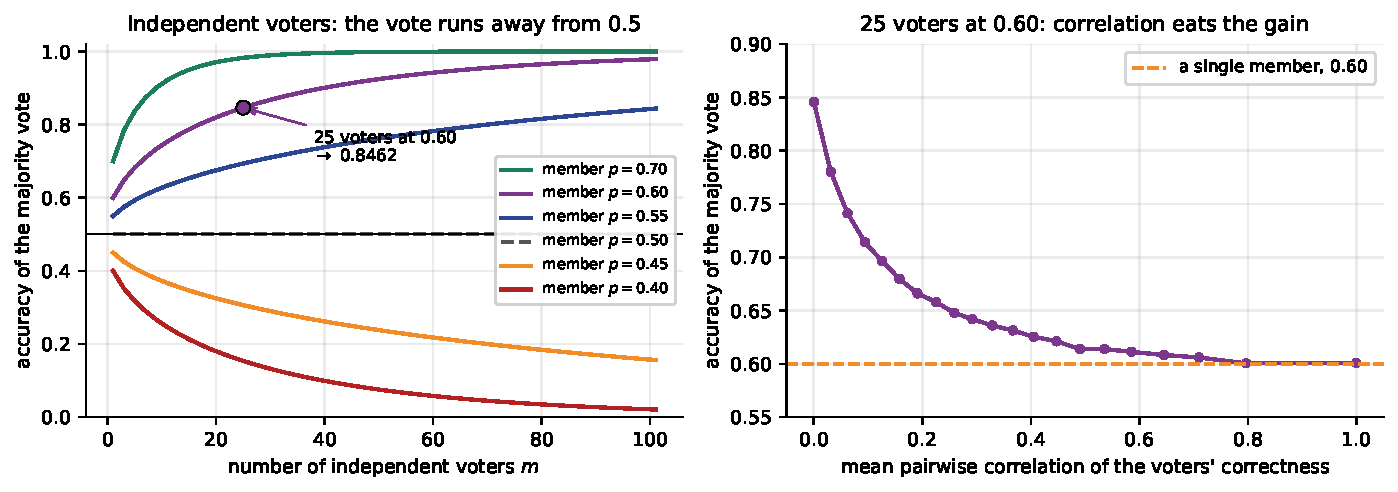
\includegraphics[width=0.88\textwidth]{binomial.pdf}
  \end{center}
  \begin{center}\small
    Left: independent voters, the curves of the table above. Right: the same
    twenty-five voters at $p = 0.60$, but now correlated. \textbf{The
    left-hand panel is the advertisement. The right-hand panel is the
    contract.}
  \end{center}
\end{frame}

\begin{frame}{Predict first \#2 --- what correlation costs}
  \begin{alertblock}{Commit to a number}
    Same twenty-five voters, each still exactly $60\%$ accurate. But now their
    \emph{correctness} is correlated: the mean pairwise correlation between
    ``member $i$ was right'' and ``member $j$ was right'' is
    $\mathbf{0.13}$ --- a correlation most people would call small.

    \medskip
    \centering\large
    The independent answer was $0.846$. What is it now?
  \end{alertblock}
  \onslide<2->{
  \begin{exampleblock}{}
    \centering\large
    $\mathbf{0.6932}$ --- more than half of the gain, gone.
  \end{exampleblock}
  \begin{center}\small
    A correlation of $0.13$ throws away $0.153$ of the $0.246$ the ensemble
    had won.
  \end{center}}
\end{frame}

\begin{frame}[fragile,shrink=6]{Independence is the whole game}
  Give each voter a latent score $Z_i = \sqrt{\rho}\,W + \sqrt{1-\rho}\,E_i$
  and call the voter correct when $Z_i < \Phi^{-1}(0.6)$. The shared $W$ is
  the common cause; $\rho$ dials how much the voters agree beyond chance.
  Every voter is still right exactly $60\%$ of the time.
\begin{outblk}
 rho_latent  mean pairwise corr   ensemble accuracy   members
   0.00          +0.0001              0.8458          0.6002
   0.05          +0.0310              0.7798          0.6006
   0.10          +0.0627              0.7381          0.5993
   0.20          +0.1260              0.6932          0.5995
   0.40          +0.2595              0.6476          0.5997
   0.70          +0.4883              0.6179          0.6002
   1.00          +1.0000              0.5993          0.5993
\end{outblk}
  \begin{center}\small
    The last column never moves. \textbf{Correlation destroys the ensemble
    without touching a single member's accuracy.} At $\rho = 1$ all
    twenty-five voters are the same voter and the committee is worth exactly
    one member.
  \end{center}
\end{frame}

\begin{frame}[fragile,shrink=8]{Ensembles of classifiers: three different learners, one vote}
  Diversity does not have to come from resampling. It can come from using
  \emph{different kinds of model}.
\begin{lstlisting}
members = [("knn",  make_pipeline(StandardScaler(), KNeighborsClassifier(5))),
           ("tree", DecisionTreeClassifier(max_depth=3, random_state=0)),
           ("lr",   make_pipeline(StandardScaler(),
                                  LogisticRegression(max_iter=5000)))]
vote = VotingClassifier(members, voting="hard").fit(Xtr, ytr)
\end{lstlisting}
\begin{outblk}
knn   test accuracy 0.9474
tree  test accuracy 0.9006
lr    test accuracy 0.9591
vote  test accuracy 0.9474
mean pairwise disagreement between members 0.0702
rows where the members were not unanimous  18 of 171
\end{outblk}
  \begin{center}\small
    \textbf{Report the result you got.} The vote did \emph{not} beat the best
    member. Three members is far too few, one of them is much worse than the
    others, and on $153$ of $171$ rows all three already agree --- so the vote
    can only act on $18$ rows. Voting is not free magic.
  \end{center}
\end{frame}

% =====================================================================
\section[Bagging]{Bagging and the bootstrap}
\label{sec:bag}

\begin{frame}[shrink=7]{Bootstrap aggregating, in one paragraph}
  \begin{exampleblock}{}
    \centering
    Draw $n$ rows \textbf{with replacement} from a training set of $n$ rows.
    Fit a model. Repeat $B$ times. Vote.
  \end{exampleblock}
  \begin{columns}[T]
    \begin{column}{0.48\textwidth}
      \begin{block}{Why with replacement}
        Without replacement, drawing $n$ from $n$ gives you the training set
        back. With replacement, some rows appear twice or three times and
        some do not appear at all --- and \emph{that} is what makes the bags
        differ.
      \end{block}
    \end{column}
    \begin{column}{0.48\textwidth}
      \begin{alertblock}{Who it works for}
        Bagging helps \textbf{unstable} learners --- ones whose output changes
        a lot when the data changes a little. Deep decision trees are the
        canonical case. Bagging a linear regression is close to a waste of
        electricity.
      \end{alertblock}
    \end{column}
  \end{columns}
  \begin{center}\small
    Breiman, 1996. The name is a contraction of \textbf{b}ootstrap
    \textbf{agg}regat\textbf{ing}.
  \end{center}
\end{frame}

\begin{frame}[fragile]{By hand: five rows, four bags}
  Training set $\{A, B, C, D, E\}$. Each bag is five draws with replacement.
\begin{outblk}
bag 1: E D C B B   in-bag unique 4/5   out-of-bag A
bag 2: A A A A E   in-bag unique 2/5   out-of-bag B,C,D
bag 3: D E C D E   in-bag unique 3/5   out-of-bag A,B
bag 4: D D C C E   in-bag unique 3/5   out-of-bag A,B
\end{outblk}
  \begin{columns}[T]
    \begin{column}{0.48\textwidth}
      \begin{block}{Read the third column}
        $4, 2, 3, 3$ distinct rows out of five --- an average of
        $3/5 = 0.60$. Every bag is a different training set; bag 2 has
        never heard of three of the five rows.
      \end{block}
    \end{column}
    \begin{column}{0.48\textwidth}
      \begin{alertblock}{Read the fourth column}
        Every bag leaves somebody out. The model trained on bag 1
        \textbf{never saw $A$ or $B$} --- so $A$ and $B$ are honest test rows
        for it, for free. Hold that thought.
      \end{alertblock}
    \end{column}
  \end{columns}
\end{frame}

\begin{frame}{Predict first \#3 --- how much of the data is in a bag?}
  \begin{alertblock}{Commit to a number}
    A training set has $n = 1000$ rows. You draw $1000$ of them with
    replacement.

    \medskip
    \centering\large
    What fraction of the original rows appears at least once?
  \end{alertblock}
  \onslide<2->{
  \begin{exampleblock}{}
    \centering\large
    $\mathbf{0.6323}$, and it is essentially the same number for every large
    $n$.
  \end{exampleblock}
  \begin{center}\small
    Most students guess something near $1.0$ (``I drew as many as I had'') or
    exactly $0.5$. The true answer is a constant of nature:
    $1 - 1/e = 0.632121$.
  \end{center}}
\end{frame}

\begin{frame}[shrink=6]{By hand: deriving $63.2\%$}
  Fix one row. On a single draw, the chance it is \emph{not} chosen is
  $1 - \tfrac{1}{n}$. The $n$ draws are independent, so
  \[
    \Pr[\text{row never chosen}] = \Bigl(1 - \frac{1}{n}\Bigr)^{n},
    \qquad
    \Pr[\text{row in the bag}] = 1 - \Bigl(1 - \frac{1}{n}\Bigr)^{n}.
  \]
  \begin{columns}[T]
    \begin{column}{0.48\textwidth}
      \begin{block}{Take the limit}
        \[
          \lim_{n\to\infty}\Bigl(1 - \frac{1}{n}\Bigr)^{n} = e^{-1}
          = 0.367879,
        \]
        so the in-bag fraction tends to
        \[
          1 - e^{-1} = \mathbf{0.632121}.
        \]
      \end{block}
    \end{column}
    \begin{column}{0.48\textwidth}
      \begin{exampleblock}{Check it at $n = 5$}
        $(1 - 1/5)^5 = 0.8^5 = 0.32768$, so the in-bag fraction is $0.67232$
        --- and the four bags on the previous slide averaged $0.60$, which
        is what four draws of a mean-$0.672$ quantity look like.
      \end{exampleblock}
      \begin{alertblock}{The consequence}
        About $\mathbf{37\%}$ of the training set is unused by each member,
        and is therefore a test set for that member.
      \end{alertblock}
    \end{column}
  \end{columns}
\end{frame}

\begin{frame}[fragile,shrink=12]{The same thing in code, and measured}
\begin{lstlisting}
rng = np.random.default_rng(0)      # the one seed for this lecture
for n in (5, 10, 50, 100, 1000, 10000):
    out = (1 - 1/n) ** n
    emp = np.mean([len(np.unique(rng.integers(0, n, n))) / n
                   for _ in range(2000)])
    print("%6d   %.6f      %.6f       %.6f" % (n, out, 1 - out, emp))
\end{lstlisting}
\begin{outblk}
  n     (1-1/n)^n     1-(1-1/n)^n    empirical unique fraction
     5   0.327680      0.672320       0.674900
    10   0.348678      0.651322       0.655600
    50   0.364170      0.635830       0.637460
   100   0.366032      0.633968       0.634460
  1000   0.367695      0.632305       0.632152
 10000   0.367861      0.632139       0.632156
limit 1 - 1/e = 0.632121
\end{outblk}
  \begin{center}\small
    Formula and measurement agree to four decimals from $n = 50$ upwards. The
    convergence is fast: by $n = 100$ you are within $0.002$ of the limit.
  \end{center}
\end{frame}

\begin{frame}{Drawn: the bootstrap fraction}
  \begin{center}
    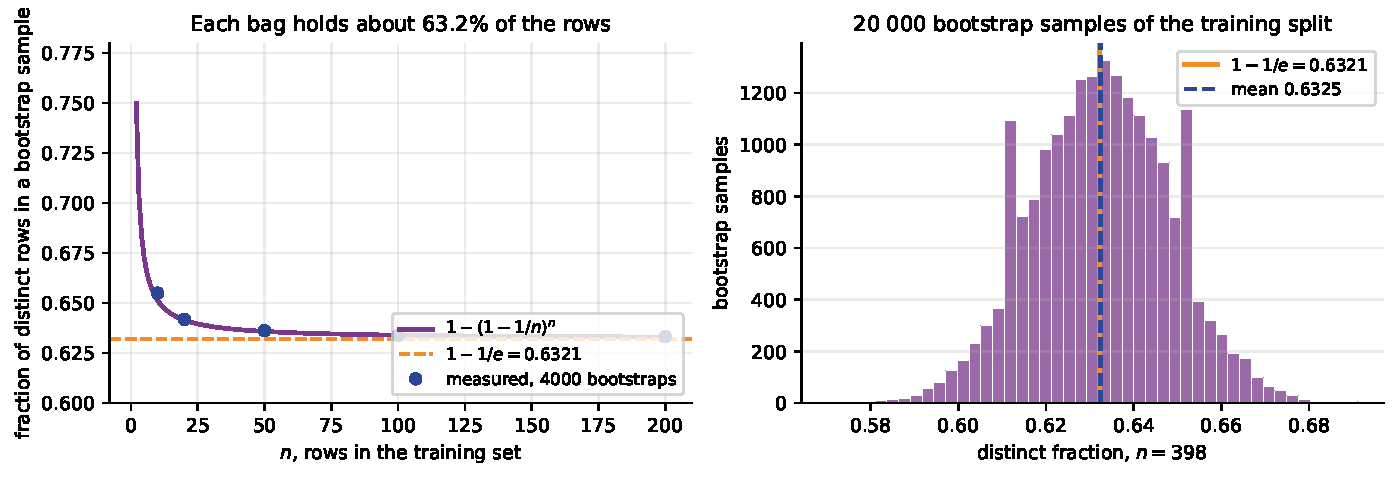
\includegraphics[width=0.90\textwidth]{bootstrap.pdf}
  \end{center}
  \begin{center}\small
    Right: twenty thousand bootstrap samples of the $398$-row training split.
    Mean $0.6325$, standard deviation $0.0158$, range $0.5704$ to $0.6910$.
    The $63.2\%$ is an average, not a guarantee --- individual bags vary by
    several percentage points.
  \end{center}
\end{frame}

\begin{frame}[fragile,shrink=5]{Bagging in code: one tree against two hundred}
\begin{lstlisting}
tree = DecisionTreeClassifier(random_state=0).fit(Xtr, ytr)
bag = BaggingClassifier(DecisionTreeClassifier(random_state=0),
                        n_estimators=200, oob_score=True,
                        random_state=0).fit(Xtr, ytr)
\end{lstlisting}
\begin{outblk}
single unpruned tree   test accuracy 0.9064
bag of 200 such trees  test accuracy 0.9298
bag out-of-bag score                 0.9598
OOB minus test                       +0.0300
5-fold CV on the training rows       0.9497
\end{outblk}
  \begin{center}\small
    \texttt{breast\_cancer}, $398$ training rows, $171$ test rows. Two hundred
    copies of a model that scores $0.9064$ give $0.9298$ --- a gain of
    $+0.0234$ with \textbf{no change to the learner at all}. Same class, same
    hyperparameters, same code.
  \end{center}
\end{frame}

\begin{frame}[shrink=5]{Out-of-bag error: a validation set you did not have to pay for}
  \begin{exampleblock}{}
    \centering
    For each training row, average only the members that \emph{did not} see it.
    Score those predictions against the truth.
  \end{exampleblock}
  \begin{columns}[T]
    \begin{column}{0.5\textwidth}
      \begin{block}{Why it is honest}
        A row is out-of-bag for about $37\%$ of the members. Those members
        never used it to choose a split. Their prediction for it is a genuine
        prediction on unseen data.
      \end{block}
      \begin{block}{Why it is free}
        No rows are held back and no model is fitted twice. Compare with
        $5$-fold cross-validation, which fits five extra ensembles.
      \end{block}
    \end{column}
    \begin{column}{0.46\textwidth}
      \begin{alertblock}{The caveat you must state}
        Each OOB prediction comes from a sub-ensemble of roughly $0.37B$
        members, not all $B$. For small $B$ that makes OOB
        \emph{pessimistic}. For $B$ in the hundreds the effect is negligible.
      \end{alertblock}
      \begin{block}{In scikit-learn}
        \texttt{oob\_score=True} on \texttt{BaggingClassifier} or
        \texttt{RandomForestClassifier}, then read \texttt{.oob\_score\_}.
      \end{block}
    \end{column}
  \end{columns}
\end{frame}

\begin{frame}[fragile,shrink=10]{Is the free estimate honest? Twenty splits say yes}
  On the single split above, OOB read $0.9598$ against a test score of
  $0.9298$ --- optimistic by $0.0300$. One split proves nothing. Repeat it.
\begin{outblk}
20 random splits of breast_cancer, forest of 300 trees
mean OOB score      0.9584  (sd 0.0054)
mean held-out score 0.9576  (sd 0.0137)
mean OOB - held-out +0.0008
paired t = 0.209, p = 0.836
\end{outblk}
  \begin{center}
    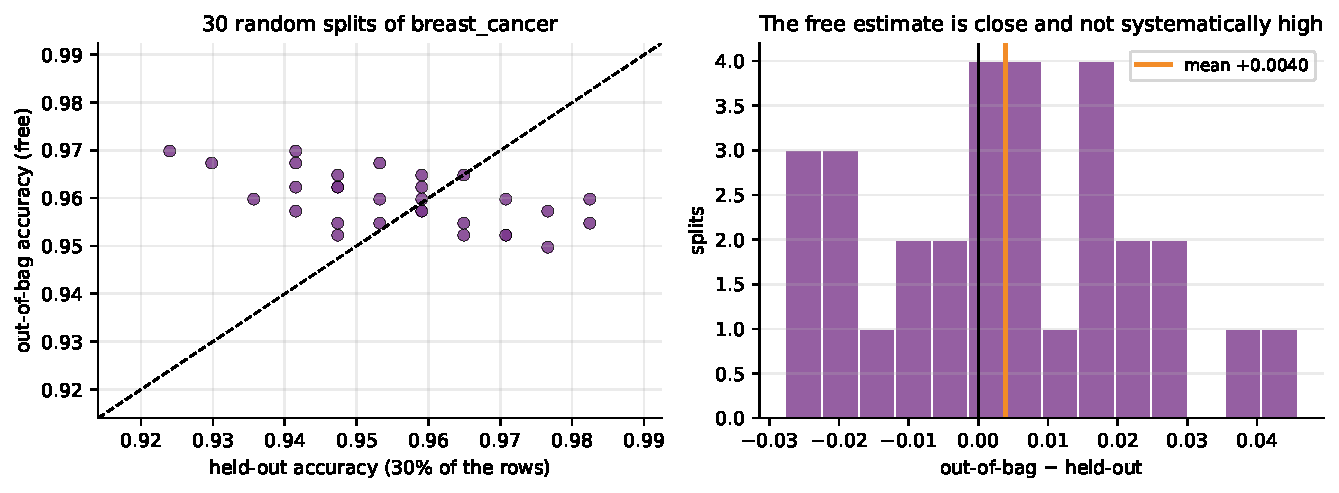
\includegraphics[width=0.62\textwidth]{oob.pdf}
  \end{center}
  \begin{center}\small
    Bias $+0.0008$, and $p = 0.836$ --- no detectable systematic
    optimism. Note the standard deviations: OOB $0.0054$ against held-out
    $0.0137$. The free estimate is not only unbiased here, it is
    \textbf{less noisy}, because it uses all $398$ rows instead of $171$.
  \end{center}
\end{frame}

% =====================================================================
\section[Variance]{Bagging reduces variance, not bias}
\label{sec:var}

\begin{frame}[shrink=18]{What averaging can and cannot fix}
  For squared-error regression the expected error at a point splits exactly:
  \[
    \mathbb{E}\bigl[(y - \hat f(x))^2\bigr]
      = \underbrace{\bigl(\mathbb{E}[\hat f(x)] - f(x)\bigr)^2}_{\text{bias}^2}
      + \underbrace{\operatorname{Var}[\hat f(x)]}_{\text{variance}}
      + \underbrace{\sigma^2}_{\text{noise}}.
  \]
  \begin{columns}[T]
    \begin{column}{0.48\textwidth}
      \begin{block}{Averaging attacks the middle term}
        The mean of $B$ things has smaller variance than one of them. It has
        \emph{the same expectation}. So bagging can only move the variance.
      \end{block}
    \end{column}
    \begin{column}{0.48\textwidth}
      \begin{alertblock}{Which is why the members should be deep}
        Use \textbf{unpruned} trees inside a bag. High variance is the thing
        bagging is good at removing; bias is the thing it cannot touch. Prune
        the members and you have thrown away the wrong half.
      \end{alertblock}
    \end{column}
  \end{columns}
  \begin{center}\small
    Measure this rather than assert it: $300$ independent training sets of
    $120$ points from $f(x) = \sin(4x) + x$ with noise $\sigma = 0.35$.
  \end{center}
\end{frame}

\begin{frame}{Drawn: three hundred training sets, two learners}
  \begin{center}
    
\includegraphics[width=0.99\textwidth]{biasvar.pdf}
  \end{center}
  \begin{center}\small
    Left and centre: forty of the three hundred fitted curves. The single
    trees scatter wildly around the truth; the bagged curves hug it. Both
    \textbf{averages} (the thick lines) sit on the dashed truth --- that is
    the bias being unchanged.
  \end{center}
\end{frame}

\begin{frame}[fragile]{The numbers behind that picture}
\begin{outblk}
single deep tree  bias^2 0.0005   variance 0.1230   bias^2+var 0.1235
bag of 50 trees   bias^2 0.0002   variance 0.0601   bias^2+var 0.0603
variance fell to 48.8% of the single tree's; bias^2 moved -0.0003
irreducible noise variance 0.1225
\end{outblk}
  \begin{columns}[T]
    \begin{column}{0.48\textwidth}
      \begin{block}{Variance: halved}
        $0.1230 \to 0.0601$. That is the entire benefit, and it is worth
        $0.0632$ of squared error per point.
      \end{block}
    \end{column}
    \begin{column}{0.48\textwidth}
      \begin{alertblock}{Bias: did not move}
        $0.0005 \to 0.0002$. Both are noise next to the variance term. A deep
        tree is nearly unbiased to begin with, so there was nothing to fix.
      \end{alertblock}
    \end{column}
  \end{columns}
  \begin{center}\small
    The noise floor is $\sigma^2 = 0.35^2 = 0.1225$. No ensemble of anything
    can go below it.
  \end{center}
\end{frame}

\begin{frame}[fragile,shrink=5]{The other half: bag a stump and watch nothing happen}
  A depth-1 stump on a sine wave is badly \textbf{biased} --- it can only
  produce two values. If bagging could fix bias, it would show here.
\begin{outblk}
single stump      bias^2 0.1856   variance 0.0281   bias^2+var 0.2137
bag of 50 stumps  bias^2 0.1842   variance 0.0147   bias^2+var 0.1989
bagging removed 48% of the stump's variance and left the bias where it was
\end{outblk}
  \begin{center}\small
    Variance halved again --- $0.0281 \to 0.0147$, the same $48\%$. And the
    bias moved by $\mathbf{0.0014}$, less than one percent of itself. Fifty
    stumps are still a stump.
  \end{center}
  \begin{alertblock}{The one-line rule}
    \centering
    \textbf{Bagging is a variance reducer. If your model is underfitting,
    bagging it will not help.} That is boosting's job, and it is why boosting
    exists.
  \end{alertblock}
\end{frame}

% =====================================================================
\section[Forests]{Random forests}
\label{sec:rf}

\begin{frame}[shrink=4]{Random forest $=$ bagging $+$ a random subset of features per split}
  \begin{exampleblock}{}
    \centering
    At \textbf{every split of every tree}, choose \texttt{max\_features}
    columns at random and search only those for the best split.
  \end{exampleblock}
  \begin{columns}[T]
    \begin{column}{0.48\textwidth}
      \begin{block}{Why bagging alone is not enough}
        If one feature is strongly predictive, \emph{every} bagged tree will
        put it at the root. The trees then look almost the same, and by the
        right-hand panel of the jury figure, an ensemble of near-identical
        members is worth barely more than one member.
      \end{block}
    \end{column}
    \begin{column}{0.48\textwidth}
      \begin{alertblock}{What the restriction buys}
        Forbid the dominant feature at some splits and those trees are forced
        to find a different structure. Each individual tree gets
        \emph{worse}. The correlation between trees falls further, and the
        ensemble gets \textbf{better}.
      \end{alertblock}
    \end{column}
  \end{columns}
  \begin{center}\small
    Defaults: $\lfloor\sqrt{d}\rfloor$ for classification, $d/3$ for
    regression. With $d = 30$, $\sqrt{30} = 5.4772$, so scikit-learn's
    \texttt{'sqrt'} uses $\mathbf{5}$.
  \end{center}
\end{frame}

\begin{frame}[shrink=10]{By hand: the variance of a correlated average}
  If $B$ members each have variance $\sigma^2$ and every pair has correlation
  $\rho$, the variance of their average is
  \[
    \operatorname{Var}\Bigl(\frac{1}{B}\sum_{b=1}^{B} T_b\Bigr)
      = \rho\,\sigma^2 + \frac{1-\rho}{B}\,\sigma^2.
  \]
  \begin{columns}[T]
    \begin{column}{0.42\textwidth}
      \begin{block}{As a fraction of $\sigma^2$, $B = 100$}
        \small
        \begin{tabular}{cc}
          \toprule
          $\rho$ & $\rho + (1-\rho)/B$ \\
          \midrule
          0.00 & 0.0100 \\
          0.10 & 0.1090 \\
          0.30 & 0.3070 \\
          0.50 & 0.5050 \\
          1.00 & 1.0000 \\
          \bottomrule
        \end{tabular}
      \end{block}
    \end{column}
    \begin{column}{0.54\textwidth}
      \begin{alertblock}{Read the first term}
        $\rho\sigma^2$ does \textbf{not} contain $B$. Adding trees drives the
        second term to zero and leaves the first one exactly where it was.

        \smallskip
        At $\rho = 0.5$, a thousand trees and a hundred trees are both stuck
        at half the variance of one tree.
      \end{alertblock}
      \begin{exampleblock}{So the only lever left}
        Once $B$ is large, the \emph{only} way to reduce the variance further
        is to reduce $\rho$. \texttt{max\_features} is the knob that does it.
      \end{exampleblock}
    \end{column}
  \end{columns}
\end{frame}

\begin{frame}[fragile,shrink=10]{Predict first \#4 --- worse trees, better forest?}
  \begin{alertblock}{Commit to an ordering}
    Three ensembles of $100$ trees on \texttt{breast\_cancer} ($d = 30$):
    plain bagging (\texttt{max\_features=30}), the default forest
    (\texttt{=5}), and one random feature per split (\texttt{=1}).
    \textbf{Rank them by \emph{ensemble} accuracy, then by \emph{average
    member} accuracy.} The two rankings are not the same.
  \end{alertblock}
\onslide<2->
\begin{outblk}
bagging (max_features=30)   tree corr 0.8261   mean single tree 0.9130   ensemble 0.9240
forest  (max_features=5)    tree corr 0.7945   mean single tree 0.9110   ensemble 0.9532
forest  (max_features=1)    tree corr 0.7010   mean single tree 0.8861   ensemble 0.9415
\end{outblk}
  \begin{columns}[T]
    \begin{column}{0.48\textwidth}
      \begin{block}{Members: monotone down}
        $0.9130 \to 0.9110 \to 0.8861$. Restricting the split search can only
        make each tree worse. It does.
      \end{block}
    \end{column}
    \begin{column}{0.48\textwidth}
      \begin{alertblock}{Ensemble: peaks in the middle}
        $0.9240 \to \mathbf{0.9532} \to 0.9415$. Correlation falls the whole
        way ($0.8261 \to 0.7010$), so the two effects trade off and the
        optimum is interior.
      \end{alertblock}
    \end{column}
  \end{columns}
  \begin{center}\small
    \texttt{max\_features=1} decorrelates the most but the trees have become
    too weak to carry the vote. This trade-off is the entire design of a
    random forest, and it is why the default is a \emph{small} number, not $1$
    and not $d$.
  \end{center}
\end{frame}

\begin{frame}[fragile,shrink=10]{Drawn and tabulated: the whole \texttt{max\_features} sweep}
  \begin{center}
    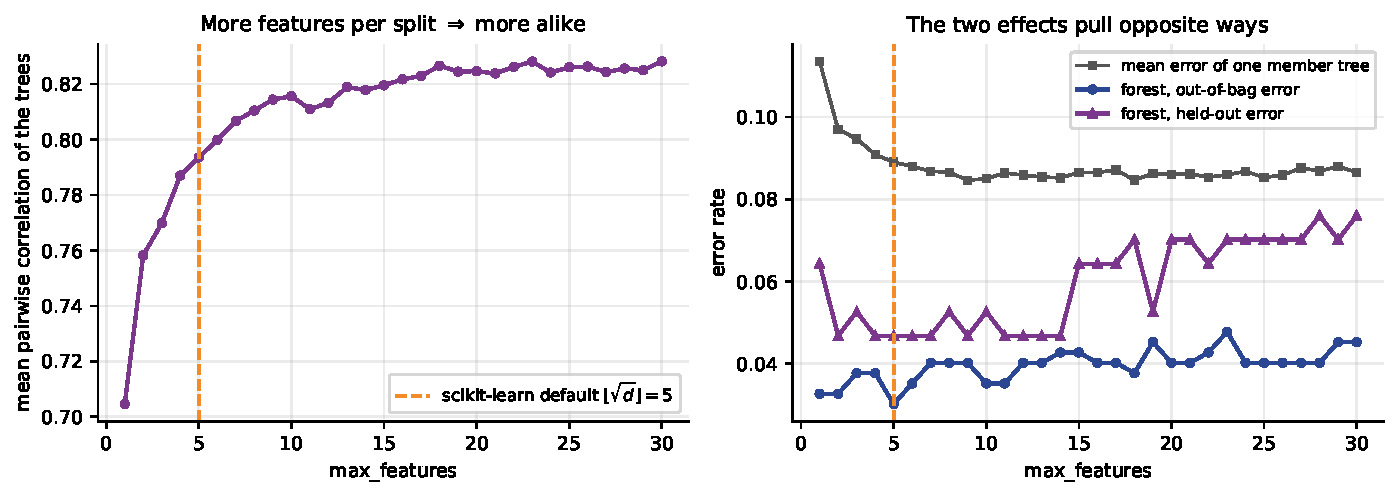
\includegraphics[width=0.86\textwidth]{maxfeatures.pdf}
  \end{center}
\begin{outblk}
 max_features   tree corr   mean single tree   OOB      test
       1         0.7046        0.8864          0.9673   0.9357
       2         0.7582        0.9030          0.9673   0.9532
       5         0.7935        0.9110          0.9698   0.9532
      12         0.8132        0.9141          0.9598   0.9532
      30         0.8282        0.9135          0.9548   0.9240
\end{outblk}
  \begin{center}\small
    OOB error is minimised at \texttt{max\_features=5} ($0.0302$) against
    $0.0452$ at $30$ --- the default is right here. And note the OOB column
    was computed \textbf{without touching the test set}: this is how you tune
    \texttt{max\_features} honestly.
  \end{center}
\end{frame}

\begin{frame}[fragile,shrink=4]{A forest is worse than every one of its trees, and better than all of them}
\begin{outblk}
a forest is 300 trees; the first three have 13, 16, 18 leaves
their individual test accuracies 0.8889 0.9123 0.8772
mean over all 300 trees          0.9120
worst single tree                0.8480
the forest                       0.9532
\end{outblk}
  \begin{columns}[T]
    \begin{column}{0.48\textwidth}
      \begin{alertblock}{No individual tree is any good}
        The average member scores $0.9120$; the worst scores $0.8480$. Every
        one of them is a small overfitted tree grown on $63\%$ of the rows
        with five features per split.
      \end{alertblock}
    \end{column}
    \begin{column}{0.48\textwidth}
      \begin{block}{The forest scores $0.9532$}
        $+0.0412$ above the average member, and above the \emph{best} of the
        three shown too. This is the jury theorem happening on real data.
      \end{block}
    \end{column}
  \end{columns}
  \begin{center}\small
    Say the sentence out loud: \textbf{the forest is better than any tree in
    it}. You cannot get that by improving a tree. You get it by having many
    that fail differently.
  \end{center}
\end{frame}

% =====================================================================
\section[Importance]{Feature importance, honestly}
\label{sec:imp}

\begin{frame}[shrink=4]{What \texttt{feature\_importances\_} actually is}
  \begin{exampleblock}{}
    \centering
    Mean decrease in impurity: for each feature, add up the impurity
    reduction of every split that used it, weighted by the rows reaching that
    split, and average over the trees.
  \end{exampleblock}
  \begin{columns}[T]
    \begin{column}{0.48\textwidth}
      \begin{block}{Why people love it}
        It is free --- the numbers fall out of the fitting. It sums to $1$. It
        needs no extra data.
      \end{block}
    \end{column}
    \begin{column}{0.48\textwidth}
      \begin{alertblock}{Why it lies}
        A column with many distinct values offers many candidate thresholds.
        More candidates means a better \emph{best} candidate, purely by
        chance. So it \textbf{systematically favours high-cardinality
        features} --- exactly the bias information gain had in the
        decision-tree lecture, now inherited by the forest.
      \end{alertblock}
    \end{column}
  \end{columns}
  \begin{center}\small
    Two demonstrations follow, deliberately of different strengths. Report
    both.
  \end{center}
\end{frame}

\begin{frame}[fragile,shrink=6]{Demonstration 1: plant three useless columns in \texttt{breast\_cancer}}
  A coin ($2$ values), a die ($6$ values) and a row identifier ($569$ values).
  All three are drawn from a random number generator and carry \textbf{no
  information whatsoever}.
\begin{outblk}
forest test accuracy with the three noise columns added 0.9357
the three planted noise columns:
   noise_uid(569)             0.0028   rank 30 of 33
   noise_dice(6)              0.0012   rank 32 of 33
   noise_coin(2)              0.0005   rank 33 of 33
the useless 569-level column scores 5.9 times the useless 2-level column
it outranks 1 of the 30 real clinical measurements
\end{outblk}
  \begin{center}\small
    \textbf{Be honest about the strength of this.} The ordering among the
    three is exactly cardinality order, $5.9\times$ from $2$ levels to
    $569$ --- the bias is real and measurable. But the thirty clinical
    measurements are genuinely strong, so the noise still lands at ranks
    $30$, $32$, $33$. On this dataset the bias distorts; it does not mislead.
  \end{center}
\end{frame}

\begin{frame}[fragile,shrink=8]{Demonstration 2: a table where it does mislead}
  Five columns, $800$ rows. \texttt{signal\_binary} agrees with $y$ $75\%$ of
  the time. \textbf{The other four are pure noise.} No model can beat
  $0.7500$; the forest gets $0.7333$.
\begin{outblk}
                     impurity   permutation
signal_binary(2)       0.2715     +0.2136  (sd 0.0294)
noise_coin(2)          0.0237     +0.0083  (sd 0.0115)
noise_dice(6)          0.0829     +0.0189  (sd 0.0131)
noise_cont(800)        0.3110     +0.0081  (sd 0.0145)
noise_uid(800)         0.3109     +0.0114  (sd 0.0127)
impurity importance puts TWO useless columns above the only informative one
useless 800-level column / useless 2-level column = 13.1 times
\end{outblk}
  \begin{center}\small
    Impurity importance ranks a \textbf{random uniform draw} and a
    \textbf{row identifier} above the only column that carries signal. A
    student who read the top of that list would delete the one useful feature
    and keep the two useless ones.
  \end{center}
\end{frame}

\begin{frame}[shrink=5]{The fix: permutation importance}
  \begin{exampleblock}{}
    \centering
    Score the fitted model on \textbf{held-out} rows. Shuffle one column.
    Score again. The drop is that column's importance. Repeat and average.
  \end{exampleblock}
  \begin{columns}[T]
    \begin{column}{0.5\textwidth}
      \begin{block}{Why it is not fooled}
        It never looks at the tree structure. It asks the only question that
        matters: \emph{if this column were destroyed, would the predictions
        get worse?} Destroying a random identifier changes nothing, so it
        scores about zero.
      \end{block}
    \end{column}
    \begin{column}{0.46\textwidth}
      \begin{alertblock}{And it gets the answer right}
        On the designed table: $\mathbf{+0.2136}$ for the signal against
        $+0.0081$ and $+0.0114$ for the two $800$-level columns. A $19\times$
        separation, in the correct direction.
      \end{alertblock}
      \begin{block}{Its own two caveats}
        Compute it on \textbf{held-out} rows, not training rows. And with
        correlated features it splits the credit --- shuffle one and the model
        reads the other.
      \end{block}
    \end{column}
  \end{columns}
\end{frame}

\begin{frame}{Drawn: the two measures side by side}
  \begin{center}
    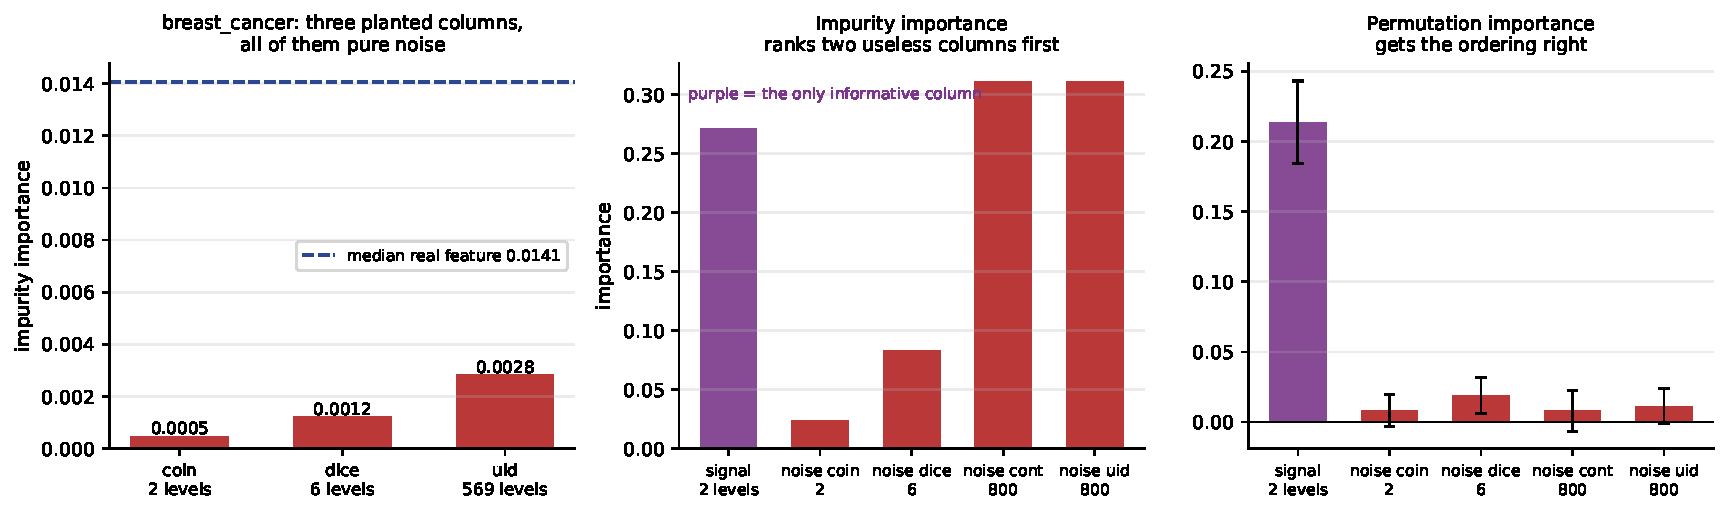
\includegraphics[width=0.99\textwidth]{importance.pdf}
  \end{center}
  \begin{center}\small
    Left: on \texttt{breast\_cancer} the three planted columns rise with
    cardinality even though all three are noise. Centre and right: on the
    designed table, impurity puts two red bars above the purple one and
    permutation does not. \textbf{Red is noise in every panel.}
  \end{center}
\end{frame}

% =====================================================================
\section[Boosting]{Boosting: AdaBoost and gradient boosting}
\label{sec:boost}

\begin{frame}[shrink=3]{Boosting inverts every design decision in bagging}
  \begin{columns}[T]
    \begin{column}{0.48\textwidth}
      \begin{block}{Bagging}
        Members are trained \textbf{in parallel} on \textbf{resampled} data,
        are \textbf{deep} (low bias, high variance), and get an
        \textbf{equal} vote.
      \end{block}
    \end{column}
    \begin{column}{0.48\textwidth}
      \begin{alertblock}{Boosting}
        Members are trained \textbf{in sequence} on \textbf{reweighted} data,
        are \textbf{shallow} (high bias, low variance), and get a
        \textbf{weighted} vote.
      \end{alertblock}
    \end{column}
  \end{columns}
  \vspace{0.4em}
  \begin{exampleblock}{The idea in one sentence}
    \centering
    Each new member is trained on a version of the data in which the rows the
    committee currently gets \emph{wrong} have been made heavier.
  \end{exampleblock}
  \begin{center}\small
    Because each member attacks the current errors, boosting reduces
    \textbf{bias}. That is the half of the decomposition bagging could not
    reach --- and it is why a boosted ensemble of \emph{stumps} works at all.
  \end{center}
\end{frame}

\begin{frame}[shrink=4]{AdaBoost, written out}
  Labels $y_i \in \{-1, +1\}$. Start with $w_i = 1/n$ for all $n$ rows. For
  $t = 1, \dots, T$:
  \begin{enumerate}
    \item Fit a weak learner $h_t$ to the data weighted by $w$.
    \item Weighted error
      $\displaystyle \varepsilon_t = \sum_{i:\, h_t(x_i) \neq y_i} w_i$.
    \item Member weight
      $\displaystyle \alpha_t
        = \tfrac{1}{2}\ln\!\Bigl(\frac{1-\varepsilon_t}{\varepsilon_t}\Bigr)$.
    \item Reweight: $w_i \leftarrow w_i\,e^{-\alpha_t y_i h_t(x_i)}$,
      then divide by the sum so the weights add to $1$.
  \end{enumerate}
  Final prediction:
  $\displaystyle F(x) = \sum_{t=1}^{T}\alpha_t h_t(x)$, classify by
  $\operatorname{sign} F(x)$.
  \begin{alertblock}{Read step 4}
    $y_i h_t(x_i) = +1$ when the member is right, so the weight is multiplied
    by $e^{-\alpha_t} < 1$ and \textbf{shrinks}. It is $-1$ when the member is
    wrong, so the weight is multiplied by $e^{+\alpha_t} > 1$ and
    \textbf{grows}. One formula does both.
  \end{alertblock}
\end{frame}

\begin{frame}[fragile,shrink=8]{By hand, round 1: ten points on a line}
  $x = 0, 1, \dots, 9$ with labels
  $y = +\,+\,+\,-\,-\,-\,+\,+\,+\,-$. Weak learner: a decision stump
  $h(x) = \pm 1$ according to $x < \theta$. All weights start at $0.1$.
\begin{outblk}
round 1: stump  h(x) = +1 if x < 2.5 else -1
   weighted error  eps = 0.3000
   alpha = 0.5*ln((1-eps)/eps) = 0.4236
   misclassified points x = 6, 7, 8
   new weights 0.0714 0.0714 0.0714 0.0714 0.0714 0.0714 0.1667 0.1667 0.1667 0.0714
\end{outblk}
  \begin{columns}[T]
    \begin{column}{0.47\textwidth}
      \begin{block}{Check $\varepsilon_1$ by hand}
        Three points wrong, each of weight $0.1$: $\varepsilon_1 = 0.3$.
        Then $\alpha_1 = \tfrac12\ln(0.7/0.3) = \tfrac12\ln 2.3333
        = \tfrac12(0.8473) = \mathbf{0.4236}$.
      \end{block}
    \end{column}
    \begin{column}{0.51\textwidth}
      \begin{alertblock}{Check the new weights by hand}
        Wrong: $0.1\,e^{0.4236} = 0.15275$, three of them. Right:
        $0.1\,e^{-0.4236} = 0.06547$, seven of them. Sum
        $= 3(0.15275) + 7(0.06547) = 0.91654$. Divide:
        $0.15275/0.91654 = \mathbf{0.1667}$ and
        $0.06547/0.91654 = \mathbf{0.0714}$.
      \end{alertblock}
    \end{column}
  \end{columns}
\end{frame}

\begin{frame}[fragile,shrink=8]{By hand, rounds 2 and 3}
\begin{outblk}
round 2: stump  h(x) = +1 if x < 8.5 else -1
   weighted error  eps = 0.2143
   alpha = 0.5*ln((1-eps)/eps) = 0.6496
   misclassified points x = 3, 4, 5
   new weights 0.0455 0.0455 0.0455 0.1667 0.1667 0.1667 0.1061 0.1061 0.1061 0.0455

round 3: stump  h(x) = -1 if x < 5.5 else +1
   weighted error  eps = 0.1818
   alpha = 0.5*ln((1-eps)/eps) = 0.7520
   misclassified points x = 0, 1, 2, 9
   new weights 0.1250 0.1250 0.1250 0.1019 0.1019 0.1019 0.0648 0.0648 0.0648 0.1250
\end{outblk}
  \begin{center}\small
    Follow the story. Round 1 fails on $6,7,8$, so round 2 arrives with those
    three heavy --- and picks a stump that gets all three right, at the price
    of $3,4,5$. Round 3 then arrives with $3,4,5$ heavy and \emph{flips
    polarity} to fix them.
    \smallskip

    Watch $\varepsilon$ fall, $0.3000 \to 0.2143 \to 0.1818$, and $\alpha$
    rise, $0.4236 \to 0.6496 \to 0.7520$. Each member is trusted more than the
    last, because each one solved a harder problem.
  \end{center}
\end{frame}

\begin{frame}{Predict first \#5 --- can three stumps beat the best stump?}
  \begin{alertblock}{Commit}
    The best single stump on these ten points misclassifies \textbf{three} of
    them, and no stump can do better --- the labels are
    $+\,+\,+\,-\,-\,-\,+\,+\,+\,-$, which no single threshold can separate.

    \medskip
    \centering\large
    How many of the ten does the weighted vote of the three stumps get right?
  \end{alertblock}
  \onslide<2->{
  \begin{exampleblock}{}
    \centering\large
    $\mathbf{10}$ of $10$. Training error zero.
  \end{exampleblock}
  \begin{center}\small
    Three models, each of which \emph{cannot} solve the problem, combine into
    one that does. This is the sense in which boosting builds a strong learner
    out of weak ones.
  \end{center}}
\end{frame}

\begin{frame}[fragile,shrink=13]{The reveal: $F(x) = \alpha_1 h_1 + \alpha_2 h_2 + \alpha_3 h_3$}
\begin{outblk}
 x      f1      f2      f3       F(x)   sign  y
 0  +1.0000 +1.0000 -1.0000  +0.3213    +1   +1
 1  +1.0000 +1.0000 -1.0000  +0.3213    +1   +1
 2  +1.0000 +1.0000 -1.0000  +0.3213    +1   +1
 3  -1.0000 +1.0000 -1.0000  -0.5260    -1   -1
 4  -1.0000 +1.0000 -1.0000  -0.5260    -1   -1
 5  -1.0000 +1.0000 -1.0000  -0.5260    -1   -1
 6  -1.0000 +1.0000 +1.0000  +0.9780    +1   +1
 7  -1.0000 +1.0000 +1.0000  +0.9780    +1   +1
 8  -1.0000 +1.0000 +1.0000  +0.9780    +1   +1
 9  -1.0000 -1.0000 +1.0000  -0.3213    -1   -1
training errors of the 3-round ensemble: 0
training errors of the best single stump: 3
\end{outblk}
  \begin{center}\small
    Check row $0$ with a pen:
    $+0.4236 + 0.6496 - 0.7520 = +0.3212$. And row $6$:
    $-0.4236 + 0.6496 + 0.7520 = +0.9780$. \textbf{Not one column of
    $f_1, f_2, f_3$ matches $y$ --- but their weighted sum does.}
  \end{center}
\end{frame}

\begin{frame}{Drawn: the weights growing and the margin appearing}
  \begin{center}
    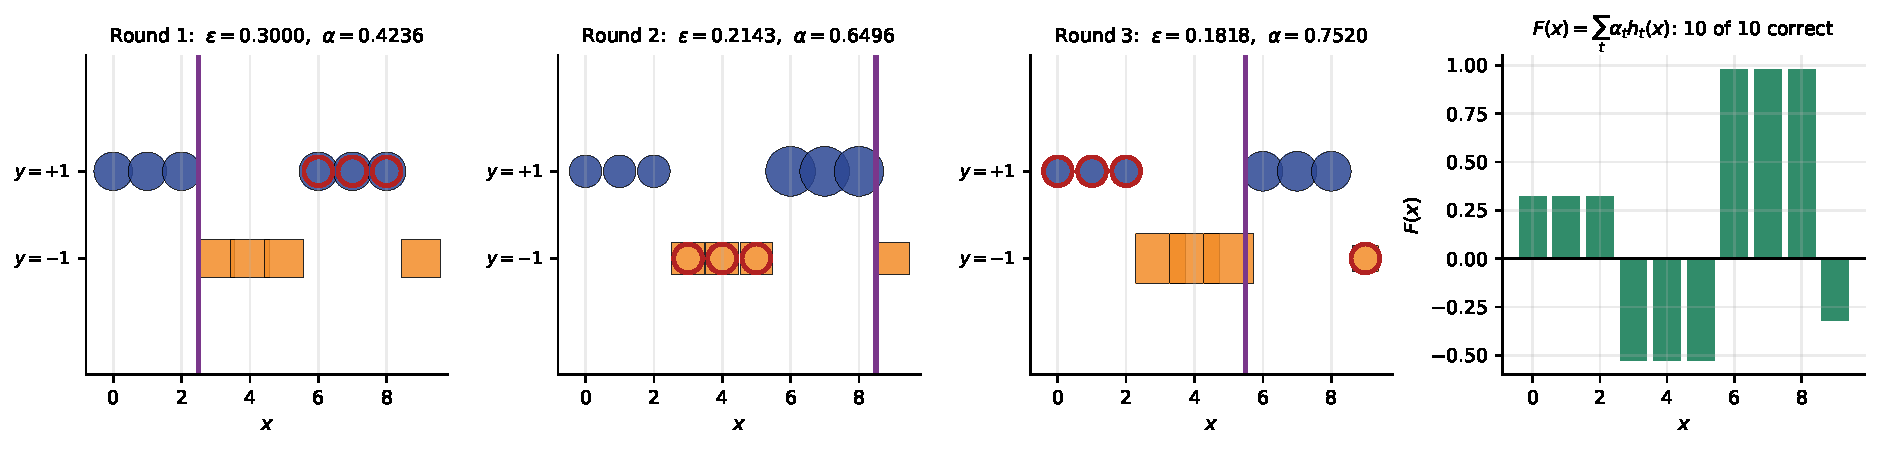
\includegraphics[width=0.99\textwidth]{adaboost.pdf}
  \end{center}
  \begin{center}\small
    Marker area is the row's weight. Red circles are the points that round's
    stump got wrong --- and they are exactly the points that grow before the
    next panel. The last panel is $F(x)$: green where the sign is right.
  \end{center}
\end{frame}

\begin{frame}[fragile,shrink=6]{And now the identical result from \texttt{AdaBoostClassifier}}
\begin{lstlisting}
ada = AdaBoostClassifier(DecisionTreeClassifier(max_depth=1, random_state=0),
                         n_estimators=3, random_state=0).fit(x[:, None], y)
\end{lstlisting}
\begin{outblk}
sklearn estimator_errors_  0.3000 0.2143 0.1818
hand-computed eps          0.3000 0.2143 0.1818
sklearn estimator_weights_ 0.8473 1.2993 1.5041
hand-computed alpha        0.4236 0.6496 0.7520
ratio sklearn/hand         2.0000 2.0000 2.0000
sklearn training errors 0, stump thresholds [2.5, 8.5, 5.5]
\end{outblk}
  \begin{center}\small
    Every $\varepsilon$ matches to four decimals and every threshold matches
    exactly. The $\alpha$'s differ by \textbf{exactly a factor of two}, every
    time: scikit-learn implements SAMME, whose weight is
    $\ln\frac{1-\varepsilon}{\varepsilon} + \ln(K-1)$, and at $K = 2$ the
    second term is $\ln 1 = 0$, leaving $2\alpha$. A constant factor on every
    member cannot change $\operatorname{sign} F$, so the predictions are
    identical.
  \end{center}
\end{frame}

\begin{frame}[fragile,shrink=11]{Gradient boosting: the same idea, with residuals instead of weights}
  For squared-error regression there is nothing to reweight --- so fit the
  next member to \textbf{what is left over}. Eight points,
  $y = 5,5,6,6,9,9,10,10$.
\begin{outblk}
stage 0: F0 = mean(y) = 7.5000
   residuals -2.500 -2.500 -1.500 -1.500 +1.500 +1.500 +2.500 +2.500
stage 1: stump on the residuals, split at x < 4.5
   stump output -2.000 -2.000 -2.000 -2.000 +2.000 +2.000 +2.000 +2.000
   F1           +5.500 +5.500 +5.500 +5.500 +9.500 +9.500 +9.500 +9.500
   SSE 2.0000
stage 2: stump on the residuals, split at x < 2.5
   F2           +5.000 +5.000 +5.667 +5.667 +9.667 +9.667 +9.667 +9.667
   SSE 1.3333
stage 3: stump on the residuals, split at x < 6.5
   F3           +4.889 +4.889 +5.556 +5.556 +9.556 +9.556 +10.000 +10.000
   SSE 1.0370
\end{outblk}
  \begin{center}\small
    $F_0$ is the mean. Every stage after it fits a stump to $y - F_{m-1}$ and
    adds it on. SSE $34 \to 2 \to 1.333 \to 1.037$.
  \end{center}
\end{frame}

\begin{frame}[shrink=6]{Drawn: fitting the residuals}
  \begin{center}
    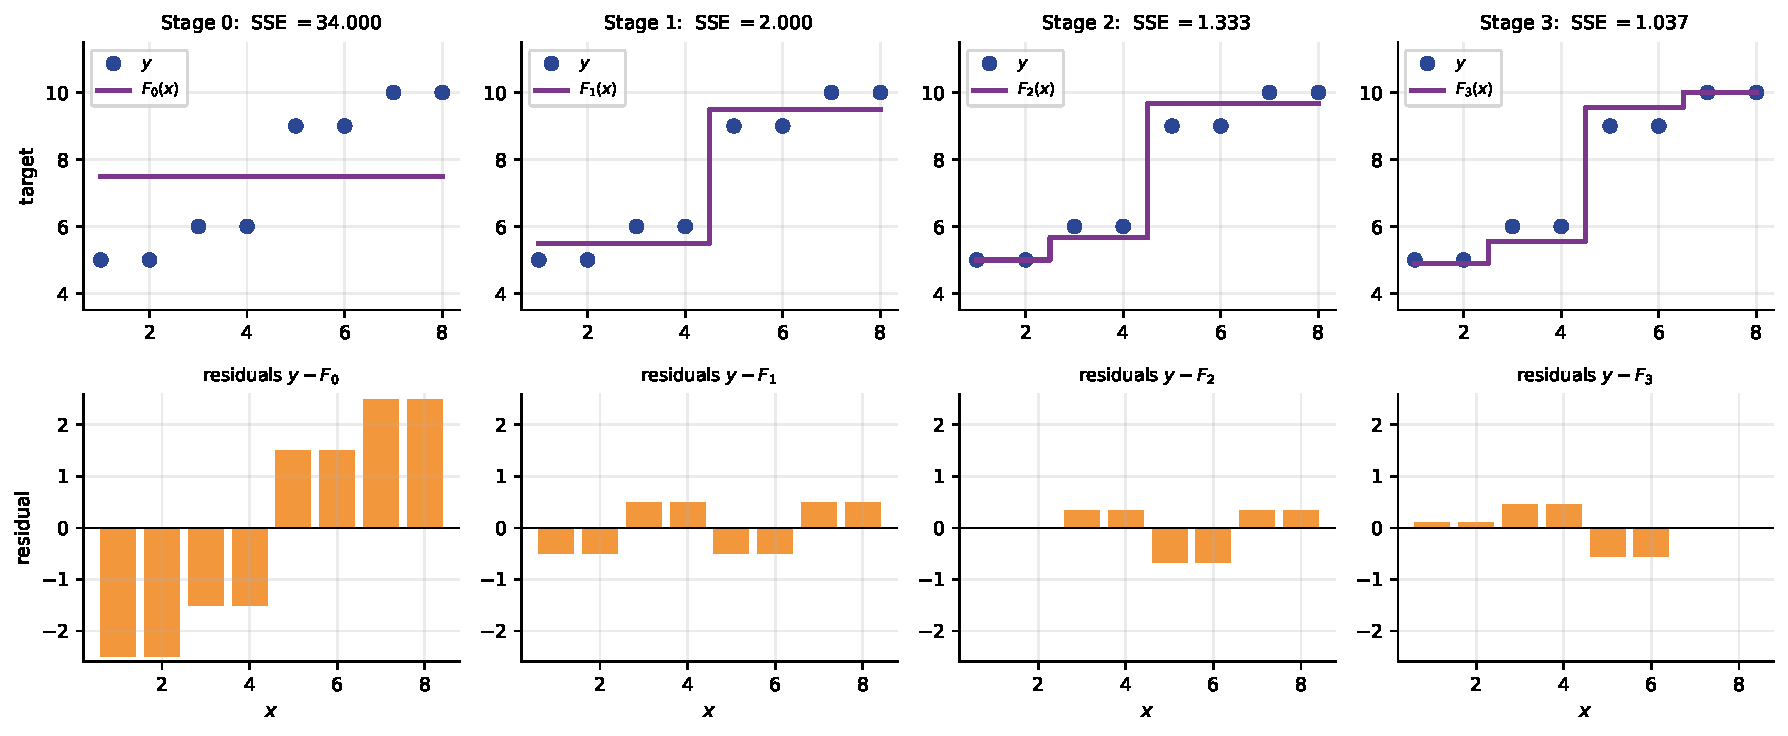
\includegraphics[width=0.82\textwidth]{gradboost.pdf}
  \end{center}
  \begin{center}\small
    Top row: the staircase $F_m$ closing on the points. Bottom row: the
    residuals it is chasing, shrinking towards zero. \textbf{Boosting is
    gradient descent in function space} --- for squared error the negative
    gradient \emph{is} the residual.
  \end{center}
\end{frame}

\begin{frame}[fragile,shrink=4]{The library does exactly that}
\begin{lstlisting}
gbm = GradientBoostingRegressor(n_estimators=3, learning_rate=1.0,
                                max_depth=1,
                                random_state=0).fit(xr[:, None], yr)
\end{lstlisting}
\begin{outblk}
sklearn init_.constant_  7.5000   (hand: mean = 7.5000)
sklearn predictions +4.889 +4.889 +5.556 +5.556 +9.556 +9.556 +10.000 +10.000
hand F3             +4.889 +4.889 +5.556 +5.556 +9.556 +9.556 +10.000 +10.000
max abs difference  0.00e+00
\end{outblk}
  \begin{alertblock}{One knob that matters more than any other}
    \texttt{learning\_rate} was set to $1.0$ here so the hand computation and
    the library agree exactly. In practice use $0.05$ to $0.1$: add
    $\eta \times$ the stump instead of the whole stump. Small steps and many
    of them generalise better than a few large ones --- and, unlike a forest,
    \texttt{n\_estimators} then becomes a parameter you must actually tune.
  \end{alertblock}
\end{frame}

% =====================================================================
\section[Bagging vs boosting]{Bagging against boosting}
\label{sec:vs}

\begin{frame}[shrink=8]{The comparison, sharply}
  \begin{center}
    \small
    \begin{tabular}{lll}
      \toprule
       & \textbf{Bagging / forests} & \textbf{Boosting} \\
      \midrule
      Members trained & in parallel, independently & in sequence, each on the
        last's errors \\
      Data each sees & a bootstrap resample & the same rows, reweighted \\
      Member depth & deep, unpruned & shallow --- stumps or depth 2--3 \\
      Vote & equal weight & weight $\alpha_t$, rises as $\varepsilon_t$ falls \\
      Attacks & \textbf{variance} & \textbf{bias} \\
      More members & plateaus, safe & can overfit, must be watched \\
      Label noise & robust --- averages it away & \textbf{fragile} --- chases it \\
      Parallelisable & yes, trivially & no, inherently sequential \\
      Tuning needed & almost none & learning rate, depth, $T$ \\
      \bottomrule
    \end{tabular}
  \end{center}
  \begin{alertblock}{The row that costs people real money}
    \centering
    A mislabelled row is a row every member keeps getting wrong. Bagging
    averages over it. \textbf{Boosting makes it heavier and heavier until the
    ensemble is built around it.}
  \end{alertblock}
\end{frame}

\begin{frame}[fragile,shrink=16]{Demonstrated: flip the training labels and watch}
  Flip a fraction of the \emph{training} labels; test on clean labels; average
  over ten splits.
\begin{outblk}
noise   RandomForest(200)   AdaBoost(200 stumps)   single tree
   0%        0.9596              0.9684            0.9322
  10%        0.9503              0.9129            0.8298
  20%        0.9368              0.8789            0.7415
  30%        0.8871              0.8240            0.6661
  40%        0.7327              0.6725            0.5637
\end{outblk}
  \begin{center}
    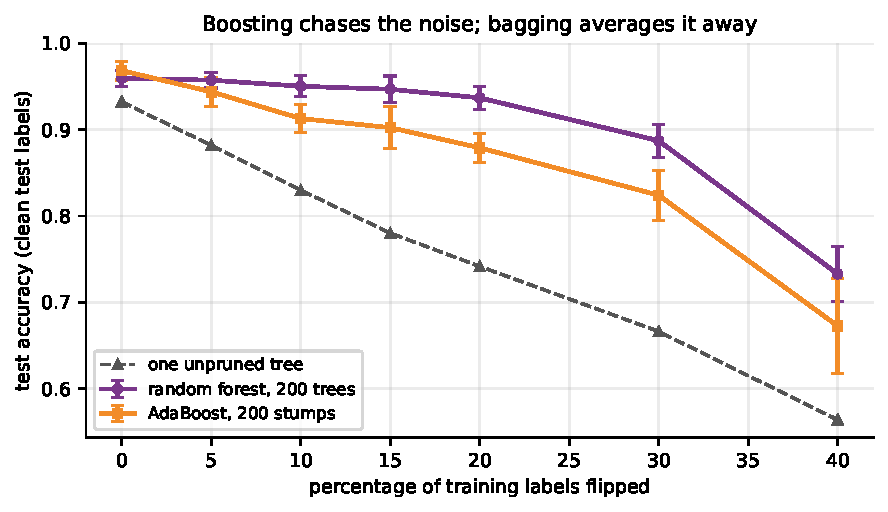
\includegraphics[width=0.52\textwidth]{noise.pdf}
  \end{center}
  \begin{center}\small
    \textbf{At $0\%$ noise AdaBoost wins} --- by $0.0088$. Say that before you
    say anything else. Then follow the columns down: by $10\%$ the forest is
    ahead by $0.0374$, and by $40\%$ by $0.0602$. Error bars are the standard
    deviation over the ten splits; both ensembles beat the single tree
    everywhere, by a wide margin.
  \end{center}
\end{frame}

\begin{frame}[fragile,shrink=9]{How many estimators? Forests plateau; boosting can turn round}
\begin{outblk}
25% of the training labels flipped
  trees     forest test acc   AdaBoost test acc
     1         0.6959            0.9006
    10         0.8129            0.9006
    50         0.9298            0.8480
   100         0.9298            0.8480
   200         0.9298            0.8129
   400         0.9298            0.8070
   800         0.9240            0.7719
forest:   best 0.9298 at T=50,  final 0.9240, drop from peak -0.0058
AdaBoost: best 0.9064 at T=19,  final 0.7719, drop from peak -0.1345
AdaBoost training accuracy at T=800: 0.9648
\end{outblk}
  \begin{center}\small
    The forest climbs and then flattens: from $T = 50$ to $T = 800$ it moves
    by $0.0058$, which is one test row. AdaBoost peaks at $T = 19$ and then
    loses $\mathbf{0.1345}$ --- while its \emph{training} accuracy climbs to
    $0.9648$ on labels that are $25\%$ wrong. That is the definition of
    overfitting.
  \end{center}
\end{frame}

\begin{frame}[fragile,shrink=7]{And on clean labels, so the comparison is fair}
\begin{outblk}
clean labels, same split
AdaBoost: best 0.9766 at T=324, final 0.9591, drop from peak -0.0175
forest:   best 0.9532 at T=100, final 0.9415, drop from peak -0.0117
\end{outblk}
  \begin{center}
    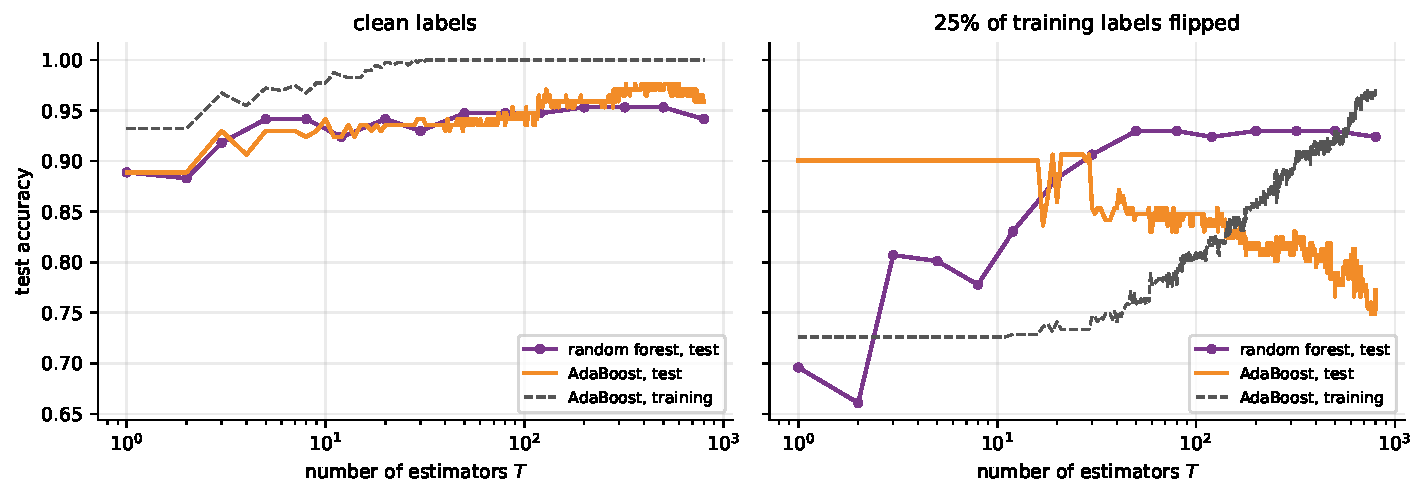
\includegraphics[width=0.78\textwidth]{nestimators.pdf}
  \end{center}
  \begin{center}\small
    On clean data AdaBoost reaches $0.9766$, above the forest's $0.9532$, and
    gives back $0.0175$ by $T = 800$; the forest gives back $0.0117$ from its
    own peak. \textbf{Two or three test rows each --- jitter, not a trend.}
    The difference is the shape: the forest is flat from $T = 50$ on both
    panels, AdaBoost falls by $0.1345$ on the noisy one and is still falling.
  \end{center}
\end{frame}

\begin{frame}[fragile,shrink=6]{All five, on three bundled datasets, five-fold cross-validated}
\begin{outblk}
                      wine     breast     digits
single tree         0.9273     0.9262     0.8592
bagging 200         0.9608     0.9579     0.9533
forest 200          0.9832     0.9667     0.9766
AdaBoost 200        0.9665     0.9754     0.8458
grad boosting       0.9494     0.9649     0.9655
\end{outblk}
  \begin{columns}[T]
    \begin{column}{0.44\textwidth}
      \begin{block}{Every ensemble beats the tree}
        On every dataset, with one exception --- and the exception is the
        interesting part.
      \end{block}
    \end{column}
    \begin{column}{0.52\textwidth}
      \begin{alertblock}{AdaBoost on \texttt{digits}: $0.8458$}
        \emph{Below} the single tree. Ten classes, and SAMME needs
        $\varepsilon_t < 1 - 1/K = 0.9$ every round; a stump on a
        ten-class problem is barely above chance. \textbf{Boosted stumps
        are a two-class instrument.}
      \end{alertblock}
    \end{column}
  \end{columns}
  \begin{center}\small
    A random forest with default settings is top or near-top on all three and
    needed no tuning at all. That is why it is the standard first thing to try
    on tabular data.
  \end{center}
\end{frame}

% =====================================================================
\section{Summary}
\label{sec:summary}

\begin{frame}[shrink=22]{Summary --- twelve lines}
  \begin{enumerate}\small
    \item An ensemble trains many models and combines them. It helps only
      when the members are \textbf{better than chance} and
      \textbf{make different mistakes}.
    \item Twenty-five \emph{independent} voters at $p = 0.60$ vote correctly
      with probability $\mathbf{0.846232}$, a gain of $+0.2462$. Below
      $p = 0.5$ the same machinery makes things worse: $0.40 \to 0.0209$ at
      $101$ voters.
    \item Correlation destroys that gain without touching any member's
      accuracy: mean pairwise correlation $0.126$ drops the vote from
      $0.8458$ to $\mathbf{0.6932}$; at correlation $1$ it is $0.5993$.
    \item A bootstrap sample of $n$ from $n$ contains
      $1 - (1-1/n)^n \to 1 - 1/e = \mathbf{0.632121}$ of the rows. Measured at
      $n = 10\,000$: $0.632156$.
    \item The other $37\%$ is the \textbf{out-of-bag} set --- free validation.
      Over $20$ splits, OOB minus held-out was $\mathbf{+0.0008}$
      ($p = 0.836$), with \emph{smaller} standard deviation than the held-out
      score.
    \item Bagging attacks variance only. $300$ resamples: variance
      $0.1230 \to \mathbf{0.0601}$, bias$^2$ $0.0005 \to 0.0002$. Bagging
      fifty \emph{stumps} halved the variance and left bias$^2$ at
      $0.1856 \to 0.1842$.
    \item $\operatorname{Var}(\bar T) = \rho\sigma^2 + \frac{1-\rho}{B}\sigma^2$.
      The first term has no $B$ in it, so once $B$ is large the only remaining
      lever is $\rho$.
    \item A forest pulls $\rho$ down with \texttt{max\_features}:
      $0.8261 \to 0.7945 \to 0.7010$ for $30, 5, 1$ features. Members get
      \emph{worse} ($0.9130 \to 0.8861$) and the ensemble peaks in the middle
      at $\mathbf{0.9532}$. Mean member $0.9120$, worst member $0.8480$,
      forest $0.9532$.
    \item Impurity importance is biased towards high-cardinality columns. On
      a designed table, two \textbf{pure-noise} $800$-level columns
      ($0.3110$, $0.3109$) outranked the only informative one ($0.2715$).
      Permutation importance on held-out rows got it right:
      $\mathbf{+0.2136}$ against $+0.0081$ and $+0.0114$.
    \item AdaBoost on ten points: $\varepsilon = 0.3000, 0.2143, 0.1818$ and
      $\alpha = 0.4236, 0.6496, 0.7520$. Three stumps that each get three
      points wrong combine to get $\mathbf{10}$ of $10$ right. scikit-learn
      reproduces every $\varepsilon$ and every threshold; its weights are
      exactly $2\alpha$ because SAMME uses
      $\ln\frac{1-\varepsilon}{\varepsilon}$.
    \item Gradient boosting fits the residuals: $F_0 = 7.5$, then stumps on
      $y - F_{m-1}$, SSE $34 \to 2 \to 1.333 \to \mathbf{1.037}$, matching
      \texttt{GradientBoostingRegressor} to $0.00\mathrm{e}{+00}$.
    \item Label noise separates them. At $0\%$ AdaBoost wins by $0.0088$; at
      $40\%$ the forest wins by $\mathbf{0.0602}$. With $25\%$ flipped labels
      AdaBoost peaks at $T = 19$ then loses $0.1345$ while its training
      accuracy climbs to $0.9648$. The forest's peak-to-final drop is
      $0.0058$, one test row.
  \end{enumerate}
\end{frame}

\begin{frame}[shrink=3]{Before the next lecture}
  \begin{columns}[T]
    \begin{column}{0.48\textwidth}
      \begin{block}{Read}
        \texttt{notes.pdf} --- the jury theorem derived, the bootstrap
        derived, three rounds of AdaBoost with every multiplication shown,
        and \textbf{practice questions with full worked solutions}.
      \end{block}
      \begin{block}{Do}
        Reproduce the three AdaBoost rounds with a pen: $\varepsilon_t$,
        $\alpha_t$, the reweighting, the normalisation, and
        $\operatorname{sign} F(x)$ for all ten points. Then compute
        $1 - (1-1/n)^n$ for $n = 5$ and $n = 10$ and say why the two answers
        are so close.
      \end{block}
    \end{column}
    \begin{column}{0.48\textwidth}
      \begin{exampleblock}{The habit to take away}
        On tabular data, fit a random forest with default settings
        \textbf{first}. It needs no scaling, no tuning and no held-out set
        (use \texttt{oob\_score=True}), and it tells you immediately what
        accuracy is achievable. Everything else is measured against it.
      \end{exampleblock}
      \begin{alertblock}{And the habit to unlearn}
        Do not read \texttt{feature\_importances\_} and believe it. Compute
        permutation importance on held-out rows before you delete a column
        or write a sentence about which variables matter.
      \end{alertblock}
    \end{column}
  \end{columns}
  \begin{center}
    \small Materials: \texttt{\AMLRepoURL}
  \end{center}
  \slidesources{\AMLUnitVISources}
\end{frame}

\end{document}
